\chapter{Regression fits differently than classification}
\label{chap:metrics}

In this chapter we compare how classification and regression differ in the way they fit the data. The results here are focused on the technical distinctions, and not on the theoretical considerations. In chapter \ref{chap:time_is_represented} we show that both methods are able to extract relevant information. The present chapter, alternatively, focuses on bringing about their most explicit distinctions. 


\begin{figure}[ht]
    \centering
    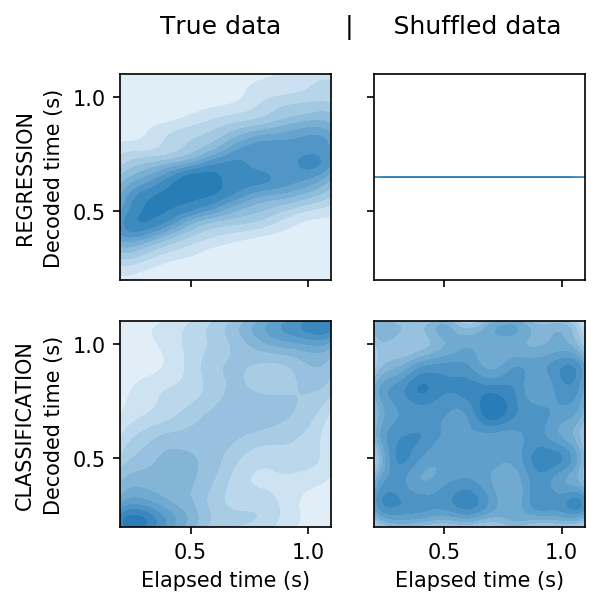
\includegraphics{figures/decoding_kde_bootstrap_vs_true_31.png}
    \caption[Comparison of prediction distributions when data is shuffled]{Comparison of prediction distributions when data is shuffled. Lines refer to the type of algorithm used to assess activity - regression and classification, while columns refer to the type of data - shuffled or not. Darker blues indicate higher density of points. For a given elapsed time, the vertical upon it is the distribution of all predictions calculated over neural activity extracted at that time.}
    \label{fig:decoding_kde_boot}
\end{figure}

To compare our decoding results, we look into the distribution of predictions according to the elapsed time of the activity. We can see the full distribution by kernel-density-estimation in figure \ref{fig:decoding_kde_boot}, and a simpler version with mean and variance in figure \ref{fig:decoding_line_boot}. When decoding shuffled data, the regression cannot find information and always predicts the mean, because this minimizes the expected root squared error. This appears in either plot as a single line located at the mean. Classification has no such strategy, because to the classifier there is no "error size" with respect to the predicted class: predicting a .2 and predicting a .9 are equal-sized errors to an example labeled .3. The mean prediction for each time bin, shown in \ref{fig:decoding_line_boot} is located around in the mean value, and distinguishes from the regression results mainly by the huge error bounds. In figure \ref{fig:decoding_kde_boot}, the prediction randomness caused by shuffling is revealed by the multiple density blobs haphazardly located. By repeating the analysis (not shown here), although the other subplots keep the same appearance, the shuffled classification changes considerably, with the blobs in other locations.

\begin{figure}[ht]
    \centering
    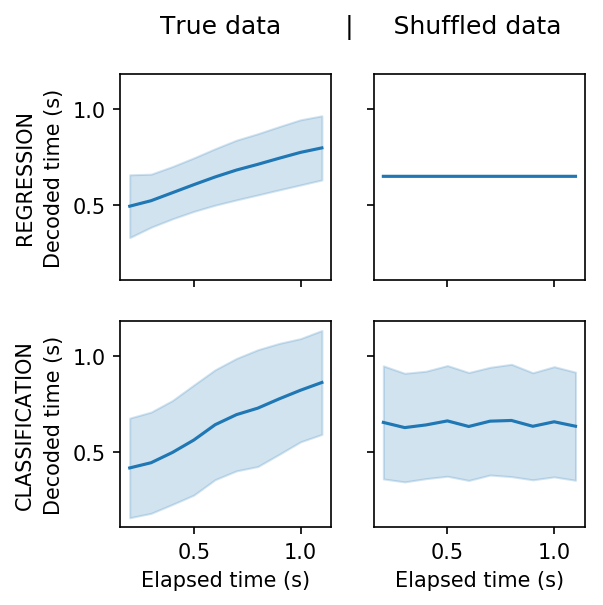
\includegraphics{figures/decoding_line_bootstrap_vs_true_31.png}
    \caption[Summary of prediction distributions comparing when data is shuffled]{Summary of prediction distributions comparing when data is shuffled. Lines refer to the type of algorithm used to assess activity - regression and classification, while columns refer to the type of data - shuffled or not. The darker line is the average decoded value for all data points extracted from a given Elapsed Time. The bands represent the standard deviation around that average.}
    \label{fig:decoding_line_boot}
\end{figure}

With respect to the true data, we can see in \ref{fig:decoding_line_boot} that the mean prediction has a positive inclination, showing that activity from later in the trial is predicted in average with higher values. While this is seen both in classification and regression, they have distinct patterns of errors, showed in \ref{fig:decoding_kde_boot}, with regression tending towards the mean values while classification tends towards the borders. The classification line has a steeper inclination, but also much bigger deviations. 

Classifiers in this task are typically better at predicting the borders of trial (onset and offset), as found in other experiments of our group. This may be an artifact of the number of proximal bins to the one being tested. Specifically, we hypothesize that, because border bins have only one proximal bin -- the previous one for the last bin, and the next one for the first bin -- they are easier to get right. All the other bins in the trial have both previous and next. Regressors, distinctly, having an error measure that is continuous and relates to the distance, do not suffer from the same artifact.

With respect to the metrics we have chosen to compare the models, something very distinct appears as a result of this "strategy" difference. When looking at the Pearson's r between the true labels and predictions, classifiers are comparable to regressors. On the other hand, when we choose to look at the explained variance, we see a huge difference. This is because the classifiers create variance in the residuals when they predict the borders. Regressors, distinct from classifiers, optimize explicitly for the sum of squared errors that gives raise to the residual variance.
